\documentclass[10pt,letterpaper]{article}
% Supplementary material (RECOMB 2027: appendix submitted as a single separate PDF).
\usepackage[letterpaper,margin=1in]{geometry}
\usepackage[T1]{fontenc}
\usepackage{mathptmx}
\usepackage{graphicx,booktabs,amsmath,amssymb,tabularx,xcolor,microtype,float}
\usepackage[font=normalsize,labelfont=bf,skip=4pt]{caption}
\usepackage[numbers,sort&compress]{natbib}
\usepackage[hidelinks]{hyperref}
\usepackage{authblk}
\renewcommand\Authfont{\normalsize}
\renewcommand\Affilfont{\normalsize}
\graphicspath{{../figures/}{../posthoc/confirm/}}
\setlength{\emergencystretch}{2em}   % long \texttt paths
\renewcommand{\thesection}{S\arabic{section}}
\renewcommand{\thefigure}{S\arabic{figure}}
\renewcommand{\thetable}{S\arabic{table}}

\title{Supplementary material for\\
``When can a small proteomics study trust its cross-validated AUC?\\
A null-calibration condition and a pre-specified benchmark''}
\author[1]{Chong Chi Yang}
\author[1]{Ong Huey Fang}
\author[2]{Michelle Yap Khai Khun}
\affil[1]{School of Information Technology, Monash University Malaysia, Bandar Sunway, Malaysia}
\affil[2]{School of Science, Monash University Malaysia, Bandar Sunway, Malaysia}
\date{}

\begin{document}
\maketitle

\section{The fusion network}\label{sup:fus}
FUS is the model of the earlier analysis, re-implemented from its code with the changes below (\texttt{vendor/fusion}
in the repository). Each input protein $j$ carries a fixed embedding $e_j \in \mathbb{R}^{480}$: the
beginning-of-sequence representation in the final (12th) layer of ESM-2 \texttt{esm2\_t12\_35M\_UR50D}
\citep{lin2023esm2}, computed once and never trained, from the protein's Ensembl peptide in the CPTAC tasks
(its UniProtKB/Swiss-Prot sequence where none maps; 13,099 of 13,290 sequences in B1 and 11,823 of 12,012 in
B2 are Ensembl peptides) and from its UniProtKB/Swiss-Prot sequence in ProCan-DepMapSanger; sequences longer than 4,000 residues were truncated (183 of
33,817 protein entries). The abundance $z_{ij}$ of protein $j$ in sample $i$ passes through an encoder
$g$ = Linear(1, 128)--ReLU--Linear(128, 480), and the two are combined additively,
$f_{ij} = e_j + \sigma(g(z_{ij}))$, with the logistic function $\sigma$ squashing the abundance encoding (the
original code calls it a gate, but it is added, not multiplied). An attention scorer
Linear(480, 128)--tanh--Linear(128, 1), softmax-normalised over the proteins of the sample, gives weights
$a_{ij}$ and the sample vector $v_i = \sum_j a_{ij} f_{ij}$, and a classifier
Linear(480, 256)--ReLU--Dropout(0.5)--Linear(256, 2) gives the logits: 247,523 trainable parameters. Training
follows the earlier analysis: unweighted cross-entropy, RMSprop (learning rate $10^{-4}$, weight decay
$10^{-4}$), 1,000 epochs, batch size 1 with the order reshuffled every epoch, prediction from the final epoch.
The earlier analysis used three classes, all 2,841 proteins and mixed precision; here the head is binary, the
input is the reference pipeline's 500 in-fold proteins (restricted to proteins with a sequence), and training
is in fp32. Fits with the same training size are stacked into one batched model in which every fit sees its
own sample at each step and receives its own loss term; since RMSprop acts elementwise, each fit gets the
update it would get alone. Against independently trained single models (four models, 200 steps, fp32, dropout
off, same initialisation and sample order) the batched logits agreed to $7.2 \times 10^{-7}$
(\texttt{prereg/measurements/RESULTS.md}). The original mixed-precision three-class trainer is not
numerically comparable. The protein ranking is the attention weight averaged over the training samples.

\section{Additional figures}
\begin{figure}[H]
\centering
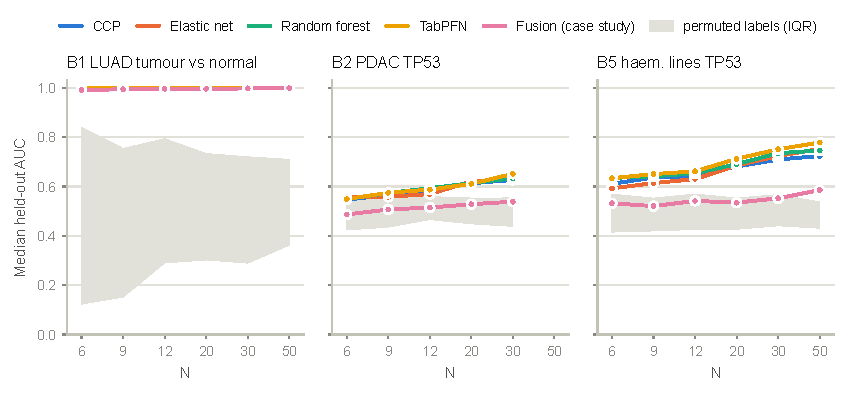
\includegraphics[width=\textwidth]{fig3_learning_curves.pdf}
\caption{Median held-out AUC by $N$, true labels; grey: interquartile range under permuted labels (B1's null
is bimodal because the cohort separates perfectly).}
\label{fig:learning}
\end{figure}

\begin{figure}[H]
\centering
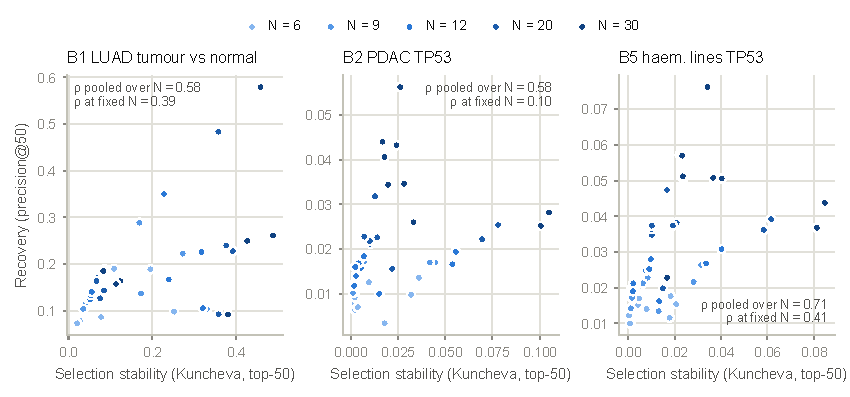
\includegraphics[width=\textwidth]{fig5_stability_vs_recovery.pdf}
\caption{Selection stability against recovery for every (configuration, $N$) cell with $N \le 30$, coloured
by $N$. The pre-specified correlation pools over $N$; within a fixed $N$ it is weak.}
\label{fig:stab}
\end{figure}

\section{Reproducibility}\label{sup:repro}
\paragraph{Runs and code versions.} Every run is one row with its seeds and a hash of the benchmark code
(\texttt{bench/*.py}). Two hashes occur. \texttt{c8068f7} produced every CPU row, 710 TabPFN rows and 1,100
fusion-network rows; \texttt{748dcfe} produced the other 2,690 TabPFN and 2,300 fusion-network rows. The two GPU
arms ran concurrently from 18:47 on 13 October 2026 until a graphics-driver reset at about 03:50 on 14 October
left both processes hung; they were resumed at 10:04, one after the other, and finished at 21:47 on
15 October (about 9\,h before and 36\,h after the interruption, 45\,h in all). The only benchmark file changed
in between was the run supervisor, \texttt{bench/supervise.py}, which gained a stall watchdog and a
keep-awake request; the runners, models and preprocessing were unchanged. Runs resume block by block, and an
unfinished block is recomputed from the start, so no run is stored twice. The hash is an MD5 over the files'
bytes as stored on the machine that ran them, where four of the 18 (\texttt{embeddings.py}, \texttt{fusion.py},
\texttt{loaders.py}, \texttt{run.py}) had Windows line endings; with those, the \texttt{bench/*.py} of commit
\texttt{8e50bbe} hashes to \texttt{c8068f7}, and the same files with \texttt{bench/supervise.py} from commit
\texttt{17be563} to \texttt{748dcfe}. The CPU arms took about 6\,h on 16 workers.

\paragraph{Re-runs.} \texttt{bench/reproduce.py} re-runs from scratch one block of every runner under each
code version, with the same units per block as the original run: two CPU blocks (B2, $N = 12$; B5, $N = 30$),
two TabPFN blocks (B1, $N = 12$, under \texttt{c8068f7}; B2, $N = 6$, under \texttt{748dcfe}) and two
fusion-network blocks of 50 repeats (B1 and B2, $N = 6$, one under each hash), 380 runs in all. Every stored
value and every protein ranking was reproduced exactly (\texttt{results/logs/reproduce.log}). The fusion network's batched trainer draws its shuffles per batch, so
a fit's result depends on which other fits share its batch. The post hoc re-runs of its pooled-LOOCV folds
(\texttt{bench/fusion\_lpo.py}; first 25 repeats of each of 13 cells) were batched differently: they matched
the stored internal AUC exactly in 87\% of 325 draws (all at $N = 6$, 94\% at $N = 9$, 72\% at $N = 12$),
differed by up to 0.05 at $N = 9$ and 0.11 at $N = 12$, and the mean absolute difference per cell was at most
0.015 (signed mean at most 0.011).

\paragraph{Leakage-test bootstrap.} The false-alarm probabilities of \S2.2 use the gate's own runs: B1,
permuted labels, 100 repeats; at $N = 12$ the leave-pair-out AUC of the 12 in-fold configurations that had a
leave-pair-out pass, at $N = 20$ the $k$-fold AUC of the 13 in-fold configurations (25 checks). Each check was
shifted so that its mean is exactly 0.5. A bootstrap replicate resamples whole repeats with replacement, the
same repeats for every configuration at a given $N$, so the correlation between configurations evaluated on
the same draw is kept; the two $N$ are resampled independently. Over 20,000 replicates the pre-specified rule
(any check's median outside $0.5 \pm 0.05$) raised an alarm in 90.5\% and the amended rule (any check's mean
above 0.55) in 7.4\% (\texttt{results/analysis/review\_gate\_bootstrap.csv}).

\paragraph{Data and resources.} CPTAC data were obtained with \texttt{cptac} 1.5.14; ProCan-DepMapSanger and
Cell Model Passports files are versioned by their release dates. Reference resources were UniProtKB/Swiss-Prot
human, Ensembl 116 and Reactome 97. Counts quoted in the paper that no other output records (eligible pathway
features, truncated sequences, the batched-trainer agreement) are recomputed by \texttt{bench/review.py
provenance} into \texttt{results/analysis/review\_provenance.csv}. The post hoc analyses are in
\texttt{bench/fusion\_lpo.py} (leave-pair-out for the fusion network), \texttt{bench/case\_study.py} (the
motivating study), \texttt{bench/stability.py} (the fixed-$N$ stability diagnostic), \texttt{bench/review.py}
(the others) and \texttt{posthoc/} (the follow-up runs); \texttt{bench/selection.py} recomputes the task
selection.

\section{Task selection}\label{sup:selection}
Table~\ref{tab:selection} recomputes the pre-specified selection (main text \S3.2) with the effect statistic
of Table~1. The script is \texttt{bench/selection.py}, and every candidate, eligible or not, is listed in
\texttt{results/analysis/task\_selection.csv}. A B2 or B5 candidate is eligible if each class has at least 35
units, so that $N = 30$ leaves 20 per class in $H_r$; among eligible candidates the smallest effect is chosen.
No other CPTAC contrast and no other ProCan-DepMapSanger tissue reaches 35 units per class. The selection itself
was made once, before any model was fitted, with an earlier implementation of the statistic, which gave 0.698,
0.831, 0.855 and 1.330 for the four B2 candidates and 0.658 and 0.735 for the two B5 candidates, in the same
order.

\begin{table}[H]
\centering
\caption{Task selection. B1: largest min(\#tumour, \#NAT), ties to more samples. B2, B5: smallest effect among
eligible candidates. Units: patients (CPTAC) or donors (ProCan-DepMapSanger). Median $|d|$: over the top 100
proteins by R limma $|t|$ on the full contrast. Bold: chosen.}
\label{tab:selection}
\begin{tabular}{@{}l l l r r r@{}}
\toprule
Task & Cohort & Contrast (positive / negative) & Units & Samples & Median $|d|$ \\
\midrule
B1 & \textbf{LUAD} & \textbf{tumour / NAT} & \textbf{111 / 102} & \textbf{213} & --- \\
 & LSCC & tumour / NAT & 110 / 102 & 212 & --- \\
 & COAD & tumour / NAT & 97 / 100 & 197 & --- \\
 & PDAC & tumour / NAT & 145 / 93 & 238 & --- \\
\midrule
B2 & \textbf{PDAC} & \textbf{TP53 mutant / wild-type} & \textbf{105 / 35} & \textbf{140} & \textbf{0.77} \\
 & CCRCC & stage I / III--IV & 52 / 45 & 97 & 0.83 \\
 & LUAD & TP53 mutant / wild-type & 67 / 41 & 108 & 0.88 \\
 & BRCA & TP53 mutant / wild-type & 54 / 66 & 120 & 1.33 \\
\midrule
B5 & \textbf{Haem.\ and lymphoid} & \textbf{TP53 driver mutant / wild-type} & \textbf{99 / 64} & \textbf{163} & \textbf{0.71} \\
 & Lung & TP53 driver mutant / wild-type & 142 / 42 & 184 & 0.74 \\
\bottomrule
\end{tabular}
\end{table}

\section{Follow-up runs}\label{sup:posthoc}
\paragraph{Procedure.} After the benchmark and its analysis were complete, five follow-up runs asked what
raises held-out AUC at small $N$ (main text \S4.6). Each began with a written plan that fixed the models, the
data, the hypotheses, the decision rule and how each outcome would be read; the plan's SHA-256 hash and time
were recorded before the run started (Table~\ref{tab:posthoc}). Run $k$ used repeats $r = 100k, \dots,
100k + 99$ of the benchmark's seeded draw procedure, none of them used before, with true labels, B2 at
$N = 6, 12, 30$ and B5 at $N = 6, 12, 30, 50$. The decision rule is the benchmark's (median paired difference
$> 0.02$ and positive in at least 75\% of draws), required in both B2 and B5 at the same $N$ and evaluated at
$N = 12$ and 30; other $N$ are descriptive. CCP, EN, RF and TabPFN were refitted on the same draws by a runner
that reproduced the stored benchmark values exactly on repeats 0--9 (B2, $N = 12$; B5, $N = 30$). Before
run 1, nine variants of the fusion network were tried on the benchmark's own repeats 0--99
(\texttt{posthoc/pilots}); these pilots motivated the plans and are not evidence. The plans of runs 1--3
described those runs as outside this paper; the decision to report all five was taken after run 5, and every
hypothesis they tested is reported in Table~\ref{tab:posthoc}.

\paragraph{Models.} \emph{V3} (runs 1--2) adds a denoising front end to the fusion network of
Section~\ref{sup:fus}: each sample's 500 in-fold abundances pass through
Linear(500, 1024)--ReLU--Linear(1024, 1024)--ReLU--Linear(1024, 500), trained jointly with the classifier to
reconstruct the clean input from a copy with 25\% of entries masked (mean squared error, weight 1; no masking
at prediction), and the per-protein encoder reads the denoised abundance $\hat z_{ij}$, giving
$f_{ij} = e_j \odot \sigma(g(\hat z_{ij}))$, a product where Section~\ref{sup:fus} has a sum; everything else
is as in Section~\ref{sup:fus}. In run 1, $e_j$ is
the ESM-2 embedding. In run 2 it is either the top $d$ principal components of the ESM-2 embeddings or a
co-expression embedding, the protein's coordinates on the top $d$ singular vectors of independent data (B2:
859 tumours of eight other CPTAC cohorts; B5: 786 ProCan-DepMapSanger lines of other tissues), with
$d = 32$ or 64 and each dimension scaled to unit SD. The co-expression embedding covered on average 97\% (B2)
and 86\% (B5) of a draw's input proteins over all run-2 draws (\texttt{confirm2\_coverage.csv}); the others get
zeros. Every embedding has a \emph{shuffled} control,
its rows permuted across proteins once per task with a fixed seed: each protein keeps a distinct tag and the
embedding keeps its distribution, but the tag no longer describes that protein. A real embedding and its
control share initial weights, masks and sample order on every draw. \emph{V2} is ridge logistic regression
($C = 1$) on $[Z, ZP/\sqrt{p}]$, with $P$ the input proteins' scores on the top 32 ESM-2 principal components
and $p = 500$ input proteins. In runs 3 and 4, ridge logistic regression on $[Z, \tau ZA]$ gives protein
coefficients $\beta = \delta + \tau A u$, so $\tau$ sets how strongly $\beta$ is drawn towards the span of
$A$. In run 3, $A$ is a 32-dimensional ESM-2 or co-expression embedding or its shuffled control, divided by
$\sqrt{p}$. In run 4 (\emph{transfer-$\tau$}), $A$ is the transferred signature below, restricted to the 500
proteins the in-fold filter kept and scaled to unit norm. $\tau$ is
chosen from $\{0, 0.125, 0.25, 0.5, 1, 2, 4, 8\}$ on $S_r$ alone, by inner cross-validation with
preprocessing refitted in every inner fold (leave-pair-out for $N \le 12$, $5 \times 5$ per-fold $k$-fold for
$N \ge 20$), ties going to the smaller $\tau$.

\paragraph{Transferred signature (runs 4 and 5).} For B2, ridge logistic regression ($C = 1$) was fitted to
831 tumours (458 \textit{TP53}-mutant) of eight other CPTAC cohorts with \textit{TP53} calls (BRCA, CCRCC,
GBM, HNSCC, LSCC, LUAD, OV, UCEC); for B5, to 775 ProCan-DepMapSanger lines (535 mutant) of 23 other tissues;
labels are defined as in the task selection (CPTAC: \texttt{harmonized} calls, else \texttt{washu}; ProCan:
Cell Model Passports driver calls). Each protein was z-scored within its cohort or tissue (missing where
observed in fewer than half of its samples, then set to 0). COAD, listed in the plan, was excluded because
its proteomics are indexed by Ensembl gene rather than protein identifiers, so none of its proteins matched
under the plan's rule; four tissues with fewer than three lines could not be standardised. No sample of
either task was used. Leave-one-cohort-out AUC within the external data, for groups with at least 10 samples
per class, was 0.67--0.82 in B2 (five cohorts) and 0.68--0.95 in B5 (nine tissues). The \emph{zero-shot}
score of a held-out sample is $\beta_\mathrm{ext}^\top z$, with $z$ standardised by $S_r$'s protein means and
SDs (over proteins observed in at least half of $S_r$; missing values set to 0). The labels of $S_r$ are not
used, and those of $H_r$ only to compute the AUC. The two signatures were built once, before any run-4 draw,
and run 5 used them unchanged (SHA-256 \texttt{74061568\ldots} for B2, \texttt{0c9f62d2\ldots} for B5).

\paragraph{Results.} Table~\ref{tab:posthoc} lists every hypothesis. Permuted-label mean held-out AUC at
$N = 12$ was 0.499--0.507 for the run-1 models and 0.504--0.510 for the run-2 models, within the plans' limit
of $0.5 \pm 0.05$. In run 3, $\tau = 0$ was chosen in 52\% (ESM-2) and 57\% (co-expression) of draws with the
real embeddings and in 52\% and 49\% with their shuffled controls, and the median held-out difference between
tuned $\tau$ and $\tau = 0$ was 0.000 in every cell. In run 4, $\tau = 0$ was chosen in 42\% of draws;
transfer-$\tau$ beat ridge in B5 at $N = 30$ and 50 ($+0.022$, $+0.024$) but not in B2, and the zero-shot
score beat TabPFN at $N = 6$, 12 and 30 in both tasks, which, as a descriptive result, became run 5's
hypothesis. Restricting the signature to the 500 kept proteins weakens it on its own: used alone in that
form on the run-4 draws, its median held-out AUC at $N = 12$ was 0.57 (B2) and 0.71 (B5), against 0.70 and
0.77 for the zero-shot score on all proteins (\emph{post hoc}, \texttt{posthoc/confirm/restricted4.py}). Run 4
therefore does not show that combining the signature with a study's labels cannot help. Table~\ref{tab:zeroshot} and Figure~\ref{fig:zeroshot} give run 5.

\begin{table}[H]
\centering
\caption{Follow-up runs. Run: number and repeats. Plan: first eight hexadecimal digits of the SHA-256 of the plan file and the time it
was fixed (2026; full hashes in \texttt{posthoc/README.md}). Outcome: whether the hypothesis held at that $N$,
i.e.\ the rule was met in both B2 and B5, with the median paired difference in B2\,/\,B5 (or its range over
the embeddings tested).}
\label{tab:posthoc}
\begin{tabularx}{\textwidth}{@{}l l >{\raggedright\arraybackslash}X >{\raggedright\arraybackslash}p{1.32in} >{\raggedright\arraybackslash}p{1.32in}@{}}
\toprule
Run & Plan & Hypothesis & $N = 12$ & $N = 30$ \\
\midrule
1 & \texttt{f5beb49e} & H1: V3 with ESM-2 beats V3 with shuffled ESM-2 & no ($-0.007$\,/\,$+0.008$) & no ($-0.017$\,/\,$-0.004$) \\
100--199 & 23 Oct 00:24 & H2: V3 with ESM-2 beats TabPFN & no ($+0.002$\,/\,$-0.007$) & no ($-0.011$\,/\,$-0.039$) \\
 & & H2: V3 with ESM-2 beats V2 & no ($0.000$\,/\,$0.000$) & no ($-0.016$\,/\,$-0.026$) \\
\addlinespace
2 & \texttt{5de9321c} & H3: V3 with co-expression ($d = 32$, 64) beats its control & no ($-0.009$ to $+0.002$) & no ($-0.021$ to $+0.001$) \\
200--299 & 23 Oct 17:09 & H4: V3 with ESM-2 PCs ($d = 32$, 64) beats its control & no ($-0.007$ to $+0.003$) & no ($-0.016$ to $+0.009$) \\
 & & H5: each of the four vs TabPFN & no difference & TabPFN beats co-expression $d = 32$; others no difference \\
\addlinespace
3 & \texttt{6dc484cf} & H6: tuned $\tau$ beats $\tau = 0$ & no ($0.000$) & no ($0.000$) \\
300--399 & 24 Oct 10:10 & \quad (each of the four embeddings) & & \\
\addlinespace
4 & \texttt{ad995aff} & H7: transfer-$\tau$ beats ridge & no ($0.000$\,/\,$0.000$) & no ($0.000$\,/\,$+0.022$) \\
400--499 & 24 Oct 10:48 & H8: transfer-$\tau$ vs TabPFN & no difference & no difference \\
\addlinespace
5 & \texttt{f4e05aa9} & H9: zero-shot beats TabPFN & \textbf{yes} ($+0.108$\,/\,$+0.096$) & \textbf{yes} ($+0.092$\,/\,$+0.038$) \\
500--599 & 24 Oct 13:39 & Zero-shot beats CCP, EN and RF & \textbf{yes} ($+0.108$ to $+0.128$) & \textbf{yes} ($+0.056$ to $+0.110$) \\
\bottomrule
\end{tabularx}
\end{table}

\begin{table}[H]
\centering
\caption{Run 5: median held-out AUC over repeats 500--599, and the zero-shot score minus TabPFN (median paired
difference and share of draws above zero).}
\label{tab:zeroshot}
\begin{tabular}{@{}l r r r r r r r@{}}
\toprule
Task & $N$ & Zero-shot & CCP & EN & RF & TabPFN & Zero-shot $-$ TabPFN \\
\midrule
B2 & 6  & 0.688 & 0.555 & 0.552 & 0.565 & 0.561 & $+0.129$ (98\%) \\
   & 12 & 0.696 & 0.574 & 0.587 & 0.578 & 0.585 & $+0.108$ (93\%) \\
   & 30 & 0.708 & 0.602 & 0.612 & 0.604 & 0.618 & $+0.092$ (85\%) \\
\addlinespace
B5 & 6  & 0.754 & 0.602 & 0.611 & 0.642 & 0.652 & $+0.112$ (98\%) \\
   & 12 & 0.769 & 0.655 & 0.643 & 0.654 & 0.666 & $+0.096$ (94\%) \\
   & 30 & 0.776 & 0.707 & 0.719 & 0.714 & 0.740 & $+0.038$ (76\%) \\
   & 50 & 0.780 & 0.737 & 0.758 & 0.757 & 0.782 & $-0.003$ (45\%) \\
\bottomrule
\end{tabular}
\end{table}

\begin{figure}[H]
\centering
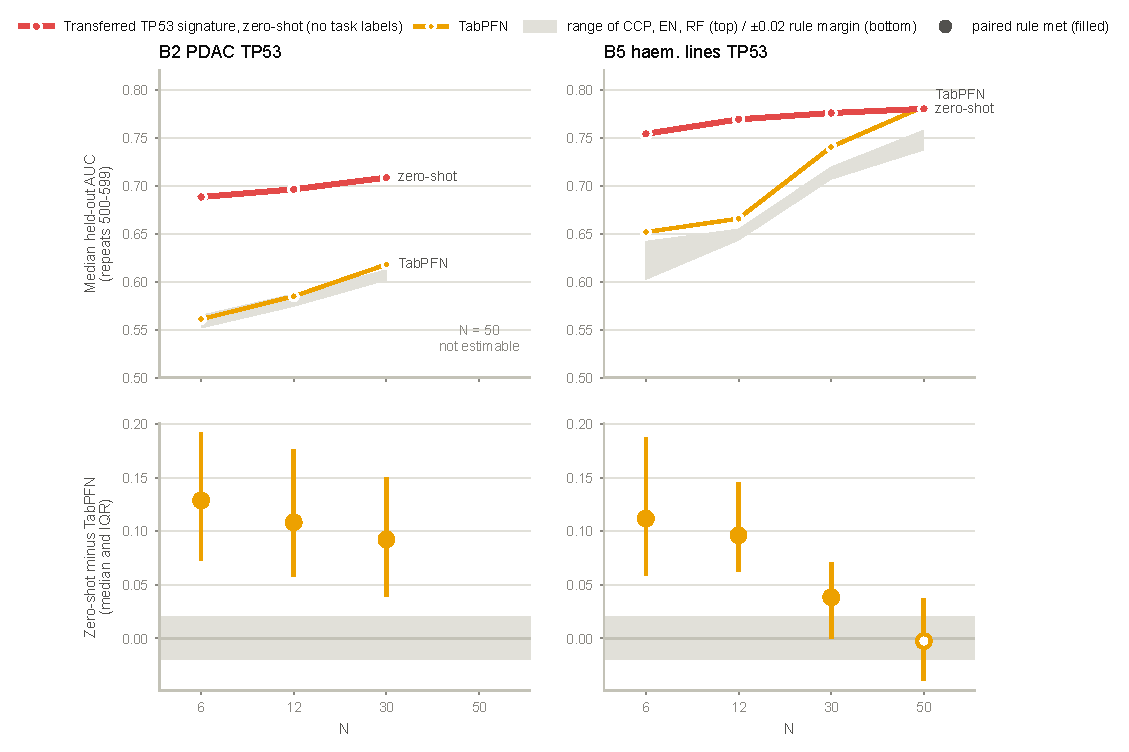
\includegraphics[width=\textwidth]{confirm5.pdf}
\caption{Run 5. Top: median held-out AUC of the zero-shot transferred signature, TabPFN, and the range of CCP,
EN and RF. Bottom: zero-shot minus TabPFN, median and interquartile range over draws; filled where the paired
rule is met in that task.}
\label{fig:zeroshot}
\end{figure}

\bibliographystyle{unsrtnat}
\bibliography{refs}

\end{document}
